\documentclass[twoside]{article}

%
% This is a borrowed LaTeX template file for lecture notes for CS267,
% Applications of Parallel Computing, UCBerkeley EECS Department.
% Now being used for CMU's 10725 Fall 2012 Optimization course
% taught by Geoff Gordon and Ryan Tibshirani.  When preparing 
% LaTeX notes for this class, please use this template.
%
% To familiarize yourself with this template, the body contains
% some examples of its use.  Look them over.  Then you can
% run LaTeX on this file.  After you have LaTeXed this file then
% you can look over the result either by printing it out with
% dvips or using xdvi. "pdflatex template.tex" should also work.
%

\setlength{\oddsidemargin}{0.25 in}
\setlength{\evensidemargin}{-0.25 in}
\setlength{\topmargin}{-0.6 in}
\setlength{\textwidth}{6.5 in}
\setlength{\textheight}{8.5 in}
\setlength{\headsep}{0.75 in}
\setlength{\parindent}{0 in}
\setlength{\parskip}{0.1 in}

%
% ADD PACKAGES here:
%

\usepackage{amsmath,amsfonts,graphicx}

%
% The following commands set up the lecnum (lecture number)
% counter and make various numbering schemes work relative
% to the lecture number.
%
\newcounter{lecnum}
\renewcommand{\thepage}{\thelecnum-\arabic{page}}
\renewcommand{\thesection}{\thelecnum.\arabic{section}}
\renewcommand{\theequation}{\thelecnum.\arabic{equation}}
\renewcommand{\thefigure}{\thelecnum.\arabic{figure}}
\renewcommand{\thetable}{\thelecnum.\arabic{table}}

%
% The following macro is used to generate the header.
%
\newcommand{\lecture}[4]{
   \pagestyle{myheadings}
   \thispagestyle{plain}
   \newpage
   \setcounter{lecnum}{#1}
   \setcounter{page}{1}
   \noindent
   \begin{center}
   \framebox{
      \vbox{\vspace{2mm}
    \hbox to 6.28in { {\bf Econ 626: Quantitative Methods II
  \hfill Fall 2018} }
       \vspace{4mm}
       \hbox to 6.28in { {\Large \hfill Lecture #1: #2  \hfill} }
       \vspace{2mm}
       \hbox to 6.28in { {\it Lecturer: #3 \hfill Scribes: #4} }
      \vspace{2mm}}
   }
   \end{center}
   \markboth{Lecture #1: #2}{Lecture #1: #2}

   %{\bf Note}: {\it LaTeX template courtesy of UC Berkeley EECS dept.}

   {\bf Disclaimer}: {\it Zhikun is fully responsible for the errors and typos appeared in the notes.}
   \vspace*{4mm}
}
%
% Convention for citations is authors' initials followed by the year.
% For example, to cite a paper by Leighton and Maggs you would type
% \cite{LM89}, and to cite a paper by Strassen you would type \cite{S69}.
% (To avoid bibliography problems, for now we redefine the \cite command.)
% Also commands that create a suitable format for the reference list.
\renewcommand{\cite}[1]{[#1]}
\def\beginrefs{\begin{list}%
        {[\arabic{equation}]}{\usecounter{equation}
         \setlength{\leftmargin}{2.0truecm}\setlength{\labelsep}{0.4truecm}%
         \setlength{\labelwidth}{1.6truecm}}}
\def\endrefs{\end{list}}
\def\bibentry#1{\item[\hbox{[#1]}]}

%Use this command for a figure; it puts a figure in wherever you want it.
%usage: \fig{NUMBER}{SPACE-IN-INCHES}{CAPTION}
\newcommand{\fig}[3]{
      \vspace{#2}
      \begin{center}
      Figure \thelecnum.#1:~#3
      \end{center}
  }
% Use these for theorems, lemmas, proofs, etc.
\newtheorem{theorem}{Theorem}[lecnum]
\newtheorem{lemma}[theorem]{Lemma}
\newtheorem{proposition}[theorem]{Proposition}
\newtheorem{claim}[theorem]{Claim}
\newtheorem{corollary}[theorem]{Corollary}
\newtheorem{definition}[theorem]{Definition}
%\newtheorem{example}[theorem]{Example}
\newenvironment{proof}{{\bf Proof:}}{\hfill\rule{2mm}{2mm}}
\newenvironment{example}{{\bf Example:}}{\hfill\rule{2mm}{2mm}}

\newtheorem{remark}[theorem]{Remark}
%\newenvironment{remark}[1][Remark]{\begin{trivlist}\item[\hskip \labelsep {\bfseries #1}]}{\end{trivlist}}


% **** IF YOU WANT TO DEFINE ADDITIONAL MACROS FOR YOURSELF, PUT THEM HERE:

\newcommand\E{\mathbb{E}}
\newcommand\dd{\mathrm{d}}

\usepackage{hyperref}
\usepackage{cancel}
\newcommand\pp{\partial}
\newcommand\imp{$\Longrightarrow$}

\begin{document}
%FILL IN THE RIGHT INFO.
%\lecture{**LECTURE-NUMBER**}{**DATE**}{**LECTURER**}{**SCRIBE**}
\lecture{4}{Calculus of Variations}{Prof. Daniel Levy}{Zhikun Lu}
%\footnotetext{These notes are partially based on those of Nigel Mansell.}
\footnotetext[1]{Visit \url{http://www.luzk.net/misc} for updates.}

\hfill Date: August 31, 2018

\section{The simplest problem of Calculus of Variations}
\begin{equation}
    \max_{x(t)} \int_{t_1}^{t_2} F(t,x(t),x'(t)) \dd t
\end{equation}
\begin{equation}
    \text{s.t.} \quad x(t_0) = x_0, x(t_1) = x_1
\end{equation}
\underline{Assumptions}
\begin{enumerate}
    \item $F(\cdots)$ is continuous in its three auguments.
    \item $F(\cdots)$ has continuous partial derivatives w.r.t. $x(t)$ and $x'(t) $.
\end{enumerate}

\begin{definition}
    A path is \underline{feasible} or \underline{admissible} if it is $C^1$ on $[t_0, t_1]$ and satisfies (4.2).
\end{definition}

\underline{FONC ({\bf Euler} Equation)}

Suppose that $x^*(t), ~t_0 \leq t \leq t_1$ solves (4.1). Let $x(t)$ be some other feasible path. Let $h(t)$ be:
\begin{equation}
     h(t) = x(t) - x^*(t)
\end{equation} 
\underline{Thus}:
\begin{itemize}
    \item $x(t)$ is a \underline{comparision} path.\\
    \item $h(t)$ is a \underline{deviation} path.
\end{itemize}
Since $x(t)$ and $x^{*}(t)$ both satisfy (4.2), we have 
\begin{equation}
    h(t_0) = h(t_1) = 0
\end{equation}

\underline{Define} $y(t)$ as follows
\begin{equation}
    y(t) = x^*(t) + a h(t)
\end{equation}
where $a$ is some parameter.

Then
\begin{equation}
    \begin{cases}
        & y(t_0) = x^*(t_0) + a h(t_0) = x^*(t_0) = x_0\\
        & y(t_1) = x^*(t_1) + a h(t_1) = x^*(t_1) = x_1
    \end{cases}
\end{equation}
It follows that $y(t)$ is a feasible path because it is $C^{1}$ for any arbitary $a$ and it satisfies (4.2).
\begin{center}
    \texttt{[insert a graph of $[x^*(t), x(t), h(t)]$ here]}
\end{center}

Hold $x^*(t)$ and $h(t)$ fixed and compute (4.1) for $y(t)$ as a function of $a$:
\begin{equation}
    \begin{aligned}
        g(a)~
        &{\buildrel \text{def} \over =} \int_{t_0}^{t_1} F(t,y(t),y'(t)) \dd t\\
        &= \int_{t_0}^{t_1} F(t,x^*(t) + a h(t),{x^*}'(t) + a h'(t)) \dd t
    \end{aligned}
\end{equation}
By assumption $x^*(t)$ maximizes (4.1). Therefore the function $g(a)$ will attain its maximum where $a = 0$. Therefore, by regular FONC,
\begin{equation}
    g'(a) \bigg |_{a = 0} = g'(0) = 0
\end{equation}

\underline{Leibnitz Theorem}

Let $f(x,r)$ be continuous w.r.t. $x, ~ \forall r$, and let $\frac{\pp f(x,r)}{\pp r}$ be continuous in the rectangle $a \leq x \leq b, ~ \underline{r} \leq r \leq \bar{r}$ in the x-r plane. Let the functions $A(r)$ and $B(r)$ be $C^1$. If $V(r) = \int_{A(r)}^{B(r)} f(x,r) \dd x$, then \begin{equation}
    V'(r) = f(B(r),r) B'(r) - f(A(r), r) A'(r) + \int_{A(r)}^{B(r)} \frac{\pp f(x,r)}{r} \dd x
\end{equation}

\underline{By Leibnitz Theorem}
\begin{eqnarray}
    g'(a) &=& ~~ F(t,x^*(t_1(a))+ a h(t_1(a)), {x^*}'(t_1(a))+ a h'(t_1(a))) \cancelto{0}{(\frac{\dd t_1}{\dd a})}\notag \\
    && -F(t,x^*(t_0(a))+ a h(t_0(a)), {x^*}'(t_0(a))+ a h'(t_0(a))) \cancelto{0}{(\frac{\dd t_0}{\dd a})}\notag \\
    && + \int_{t_0}^{t_1} \bigg [ 
    F_x(t,x^*(t)+ a h(t), {x^*}'(t)+ a h'(t)) h(t) \notag \\
    && + F_{x'}( t, x^*(t)+ a h(t), {x^*}'(t)+ a h'(t) ) h'(t)
    \bigg ] \dd t \notag \\
    &=& \int_{t_0}^{t_1} \bigg [ 
    F_x(t,x^*(t)+ a h(t), {x^*}'(t)+ a h'(t)) h(t) + F_{x'}(t,x^*(t)+ a h(t), {x^*}'(t)+ a h'(t)) h'(t)
    \bigg ] \dd t\\
    g'(0) &=& \int_{t_0}^{t_1} \bigg [ 
    F_x(t,x^*(t), {x^*}'(t)) h(t) + F_{x'}(t,x^*(t), {x^*}'(t)) h'(t)
    \bigg ] \dd t = 0 \quad \text{by FONC} 
\end{eqnarray}
which is a necessary condition for a maximum.

\underline{Note:} (4.11) must hold for all $h$ that is continuous and satisfies (4.4).

\underline{Recall:} Integration by part
\begin{eqnarray}
    \int_{t_0}^{t_1} \bigg [ 
    F_{x'}(t,x^*(t), {x^*}'(t)) h'(t)
    \bigg ] \dd t &=& [ 
    F_{x'}(t,x^*(t), {x^*}'(t)) h(t) ] {\bigg |}_{t_0}^{t_1} - \int_{t_0}^{t_1} \bigg [ 
    h(t) \frac{\dd }{\dd t}F_{x'}(t,x^*(t), {x^*}'(t)) 
    \bigg ] \dd t\\
    &=&  0 - \int_{t_0}^{t_1} \bigg [ 
    h(t) \frac{\dd }{\dd t}F_{x'}(t,x^*(t), {x^*}'(t)) 
    \bigg ] \dd t
\end{eqnarray}

\begin{eqnarray}
    g'(0) &=& \int_{t_0}^{t_1} \bigg [ 
    F_x(t,x^*(t), {x^*}'(t)) h(t) + F_{x'}(t,x^*(t), {x^*}'(t)) h'(t)
    \bigg ] \dd t\\
    &=& \int_{t_0}^{t_1} \bigg [ 
    F_x(t,x^*(t), {x^*}'(t)) h(t)
        \bigg ] \dd t + 
    \int_{t_0}^{t_1} \bigg [ 
     F_{x'}(t,x^*(t), {x^*}'(t)) h'(t)
        \bigg ] \dd t \\
    &=& \int_{t_0}^{t_1} \bigg [ 
    F_x(t,x^*(t), {x^*}'(t)) h(t)
        \bigg ] \dd t - \int_{t_0}^{t_1} \bigg [ 
    h(t) \frac{\dd }{\dd t}F_{x'}(t,x^*(t), {x^*}'(t)) 
    \bigg ] \dd t \\
    &=& \int_{t_0}^{t_1} \bigg [ 
    F_x(t,x^*(t), {x^*}'(t)) - \frac{\dd }{\dd t}F_{x'}(t,x^*(t), {x^*}'(t)) \bigg ] h(t) \dd t = 0
\end{eqnarray}
(4.17) must hold true if $x^*(t)$ maximizing (4.1). Moreover, it must hold for all $h(t)$ that is $C^1$ and satisfies (4.4). This will be true only if the term in the brackets vanishes:
\begin{equation}
    F_x - \frac{\dd }{\dd t}F_{x'} = 0, ~ t_0 \leq t \leq t_1 
\end{equation}
which is a necessary condition for a maximum. (4.18) is called \underline{Euler Equation}. The Euler equation holds true because of the following lemma.

\begin{theorem}[The Fundamental Lemma of Calculus of Variations]
    Suppose that $g(t)$ is a continuous function defined on $[t_0, t_1] $. If \begin{equation}
        \int_{t_0}^{t_1} g(t) h(t) \dd t = 0
    \end{equation} for all continuous $h(t)$ defined on $[t_0, t_1] $ and satisfies (4.4), then $g(t) = 0 ~ \forall t \in [t_0, t_1]$.
\end{theorem}
\begin{proof}
    Suppose that $g(t) \neq 0$ for some $\bar{t} \in [t_0, t_1]$. WLOG, assume $g(\bar{t}) = m >0$. Since $g(t)$ is continuous at $t = \bar{t}$, for $\epsilon = \frac{m}{2}$, we know there exist $\delta_\epsilon >0$ such that,
    \begin{equation}
        g(t) \geq g(\bar{t}) - \epsilon = m - \frac{m}{2} = \frac{m}{2}, \qquad \forall t \in (\bar{t}-\delta_\epsilon, \bar{t}+\delta_\epsilon)\cap [t_0, t_1]
    \end{equation}

    Let $h(t)$ be \begin{equation}
        h(t) = \begin{cases}
            (t-a)(b-t), &\text{ if } t \in [a,b]\\
            0, & \text{ elsewhere }
        \end{cases}
    \end{equation}
    with $a = \max \{\bar{t}-\delta_\epsilon, t_0 \}$, $b = \min \{ \bar{t}+\delta_\epsilon, t_1 \}$, and $b-a >0$ for $\delta_\epsilon$ sufficiently small. (Also note that $h(t_0) = h(t_1) = 0$ and $h(\cdot)$ is continuous.)
%    \begin{center}
%    \texttt{[insert a graph of $h(t)$ here]}
%    \end{center}
    \begin{equation}
        \int_{t_0}^{t_1} g(t) h(t) \dd t = \int_{a}^{b} g(t) (t-a)(b-t) \dd t \geq \int_{a}^{b} \frac{m}{2} (t-a)(b-t) \dd t = \frac{(b-a)^3}{6} > 0
    \end{equation}
    which contradicts the hypothesis that (4.19) holds for all $h(t)$ with the required properties.
\end{proof}

\underline{Other versions of the Euler equation}
\begin{equation}
    \frac{\dd F_{x'}}{\dd t} = F_{x't} + F_{x'x}x' + F_{x'x'} x''
\end{equation}
\begin{equation}
    \Longrightarrow F_x = F_{x't} + F_{x'x}x' + F_{x'x'} x''
\end{equation}
where the partial derivatives must be evaluated at $(t, x^*, {x^*}')$ and $x' = x'(t)$, $x'' = x''(t)$. Note also that (4.24) is a second order differential equation.

Integrate (4.18) \imp
\begin{equation}
    F_{x'} = \int F_x + C_1
\end{equation}
which is known as \underline{du Bois-Reymond} equation.

\underline{Consider}
\begin{equation}
    \frac{\dd }{\dd t}[F - x' F_{x'}] = F_{t} + F_{x}x' + \cancel{F_{x'} x''} - x' \frac{\dd F_{x'} }{\dd t} - \cancel{x'' F_{x'}} = F_t + x' \cancelto{0 \text{ by EE}}{(F_x - \frac{\dd F_{x'} }{\dd t})}
\end{equation}
\imp
\begin{equation}
    \frac{\dd }{\dd t}[F - x' F_{x'}] = F_t
\end{equation}
which is particularly useful if $F$ does not depend on $t$ directly, i.e. $F_t = 0$.

\begin{example}
    $F(\cdot)=(x'(t))^2 $
    \begin{equation}
        \begin{cases}
            \min ~ \int_0^T (x'(t))^2 \dd t\\
            \text{s.t.} \quad x(0) = 0, ~ x(T) = B
        \end{cases}
    \end{equation}
\end{example}
\begin{equation}
    F_{x'} = 2x'(t), F_x = 0
\end{equation}
EE \imp \begin{equation}
    0 = \frac{\dd }{\dd t}[2x'(t)]
\end{equation}
\begin{equation}
    \Longrightarrow x''(t) = 0
\end{equation}
\begin{equation}
    x(t) = c_1 t + c_2
\end{equation}
With $x(0) = 0, ~ x(T) = B$, we get
\begin{equation}
    x(t) = \frac{B}{T}t.
\end{equation}































































%$$##
\clearpage
\section*{References}
%\beginrefs
%\bibentry{CW87}{\sc D.~Coppersmith} and {\sc S.~Winograd}, 
%``Matrix multiplication via arithmetic progressions,''
%{\it Proceedings of the 19th ACM Symposium on Theory of %Computing},
%1987, pp.~1--6.
%\endrefs

% **** THIS ENDS THE EXAMPLES. DON'T DELETE THE FOLLOWING LINE:

\end{document}










\section{Infinite Horizon Model}
{\bf (Growth Model -- Lucas, Stokey and Prescott)}
\begin{equation}
    V(K_0) = \begin{cases}
        \max\limits_{\{C_0, K_1\}} [u(C_0)+ \beta V(K_1)]\\
        \quad s.t. \quad C_0 + K_1 = f(K_0)
    \end{cases}
\end{equation}
\begin{equation}
    \Longrightarrow V(K_0) = \max\limits_{\{ K_1\}} [u(f(K_0)-K_1)+ \beta V(K_1)]
\end{equation}

\underline{FONC}

\begin{equation}
    u'(f(K_0)-K_1) = \beta V'(K_1)
\end{equation}
By assumption
\begin{equation}
    K_1 = g(K_0)
\end{equation}
\begin{equation}
    V(K_0) = u(f(K_0)-g(K_0)) + \beta V(g(K_0))
\end{equation}
\underline{Total differential}:
\begin{equation}
    \begin{aligned}
        V'(K_0) &= u'(f(K_0)-g(K_0))(f'(K_0) - g'(K_0))+ \beta V'(g(K_0))g'(K_0)\\
        &= u'(f(K_0)-g(K_0))  f'(K_0) - [u'(f(K_0)-g(K_0))- \beta V'(g(K_0)) ]  g'(K_0)\\
        &= u'(f(K_0)-g(K_0))  f'(K_0)
    \end{aligned}
\end{equation}
Here, $[u'(f(K_0)-g(K_0))- \beta V'(g(K_0)) ]  g'(K_0) = 0$ by FONC (2.3), which follows from the envelope theorem.

\underline{Lead one period}
\begin{eqnarray}
    V'(K_1) &=& u'(f(K_1)-K_2)  f'(K_1)\\
    \Longrightarrow u'(f(K_0)-K_1) &=& \beta u'(f(K_1)-K_2)  f'(K_1)
\end{eqnarray}
which is a second order difference equation in $\mathbb{R}$.

\underline{Assumptions}
\begin{eqnarray}
    f(K_t) &=& K_t^a, \quad 0 < a < 1\\
    u(C_t) &=& \ln C_t
\end{eqnarray}

\underline{Recall}
\begin{equation}
    V(K_t) = \begin{cases}
        \max\limits_{\{C_t, K_{t+1}\}} [u(C_t)+ \beta V(K_{t+1})]\\
        \quad s.t. \quad C_t + K_{t+1} = f(K_t)
    \end{cases}
\end{equation}

\underline{Choice Variables}: $\{C_t, K_{t+1}\}_{t=0}^{\infty}$

\underline{Set up a Lagrangian}
\begin{equation}
    \mathcal{L} = u(C_t)+ \beta V(K_{t+1}) + \lambda_t [ f(K_t) - C_t + K_{t+1}]
\end{equation}
With our functional forms, it becomes
\begin{equation}
    \mathcal{L} = \ln C_t+ \beta V(K_{t+1}) + \lambda_t [ K_t^a - C_t + K_{t+1}]
\end{equation}

\underline{FONC}
\begin{eqnarray}
    &[C_t]&     \frac{1}{C_t} - \lambda_t = 0\\
    &[K_{t+1}]&  \beta V'(K_{t+1}) - \lambda_t = 0\\
    &\Longrightarrow& \frac{1}{C_t} = \beta V'(K_{t+1})
\end{eqnarray}
Apply the envelope theorem again [\texttt{Benveniste-Scheinkman Theorem}]. Suppose we have a solution of all variables as a function of the state:
\begin{eqnarray}
    C_t &=& C_t(K_t)\\
    K_{t+1} &=& K_{t+1}(K_t)\\
    \lambda_t &=& \lambda_t(K_t)
\end{eqnarray}
then (2.13) $\Longrightarrow$
\begin{equation}
    V(K_t) = \mathcal{L}^* = \ln C_t(K_t) + \beta V(K_{t+1}(K_t)) + \lambda_t [ K_t^\alpha - C_t(K_t) + K_{t+1}(K_t)]
\end{equation}
which is a function of $K_t$ only.

Differentiate w.r.t. $K_t$
\begin{eqnarray}
    V'(K_t) &=& \frac{1}{C_t(K_t)}C_t'(K_t) + \beta V'(K_{t+1})K_{t+1}'(K_t) + \lambda_t'(K_t) [ K_t^\alpha - C_t(K_t) + K_{t+1}(K_t)] + \lambda_t(K_t) [\alpha K_t^{\alpha-1}- C_t'(K_t) + K_{t+1}'(K_t)]\\
    &=& \frac{1}{C_t(K_t)}C_t'(K_t) + \beta V'(K_{t+1})K_{t+1}'(K_t) + \lambda_t(K_t) [\alpha K_t^{\alpha-1}- C_t'(K_t) + K_{t+1}'(K_t)] \quad (\text{as } K_t^\alpha - C_t + K_{t+1} = 0)\\
    &=& C_t'(K_t) \left [ \frac{1}{C_t(K_t)} - \lambda_t(K_{t}) \right ] + K_{t+1}'(K_t)[\beta V'(K_{t+1})K_{t+1}'(K_t) - \lambda_t(K_t)] + \lambda_t(K_t) \alpha K_t^{\alpha-1}\\
    &=&  \lambda_t(K_t) \alpha K_t^{\alpha-1} \qquad (\text{since the first two terms are 0 by FONC)}\\
    &=& \frac{1}{C_t(K_t)} \alpha K_t^{\alpha-1}
\end{eqnarray}
Leap one period forward
\begin{equation}
    V'(K_{t+1}) = \frac{1}{C_{t+1}(K_{t+1})} \alpha K_{t+1}^{\alpha-1} 
\end{equation}
\underline{Note}: we could obtain the same result directly from (2.12) with envelope theorem. If we take the value function of (2.12)
\begin{equation}
    V(K_t) = \max \{ u(C_t)+ \beta V(K_{t+1}) + \lambda_t [ f(K_t) - C_t + K_{t+1}] \}
\end{equation}
and ignore the dependence of $C_t$ and $K_{t+1}$, because we are at maximum point, then by the envelope theorem:
\begin{equation}
    V'(K_t) = \lambda_t f'(K_t)
\end{equation}
(2.26) and (2.16) lead to
\begin{equation}
    \frac{1}{C_t} = \beta \frac{1}{C_{t+1}}\alpha K_{t+1}^{\alpha - 1}
\end{equation}
which is a first order difference equation in $C$. Recall the budget constraint
\begin{equation}
    C_t + K_{t+1} = K_t^\alpha
\end{equation}
which is a first order difference equation in $K$. 

Note that (2.29) and (2.30) are connected. Together, they form a system of two first order difference equations.
$$\begin{cases} 
    \dfrac{1}{C_t} = \beta \frac{1}{C_{t+1}}\alpha K_{t+1}^{\alpha - 1}\\
    C_t + K_{t+1} = K_t^\alpha
\end{cases}$$


\section{Solution Methods}
Three method for solving dynamic programming problems:
\begin{enumerate}
    \item Policy function iteration
    \item Value function iteration
    \item Guess intelligently
\end{enumerate}
\subsection{Policy Function Iteration}
From (2.29), we have \begin{equation}
    \frac{K_{t+1}}{C_t} = \frac{\alpha \beta}{C_{t+1}}K_{t+1}^\alpha
\end{equation}
(2.30) $\Longrightarrow$
\begin{equation}
    1+ \frac{K_{t+1}}{C_t} = \frac{K_t^\alpha}{C_t}
\end{equation}
Together $\Longrightarrow$
\begin{equation}
    \alpha \beta \frac{K_{t+1}^\alpha}{C_{t+1}} = \frac{K_t^\alpha}{C_t} - 1
\end{equation}
which is a first order difference equation in $\dfrac{K^\alpha}{C}$.

Solve the difference equation by sucessive substitution \underline{forward}:
\begin{eqnarray}
    \frac{K_t^\alpha}{C_t} &=& 1+ \alpha \beta \frac{K_{t+1}^\alpha}{C_{t+1}}\\
    \frac{K_{t+1}^\alpha}{C_{t+1}} &=& 1+ \alpha \beta \frac{K_{t+2}^\alpha}{C_{t+2}}\\
    \frac{K_t^\alpha}{C_t} &=& 1+ \alpha \beta (1+ \alpha \beta \frac{K_{t+2}^\alpha}{C_{t+2}})\\
    \frac{K_t^\alpha}{C_t} &=& 1+ \alpha \beta  + (\alpha \beta)^2 \frac{K_{t+2}^\alpha}{C_{t+2}}\\
    \frac{K_{t+2}^\alpha}{C_{t+2}} &=& 1+ \alpha \beta \frac{K_{t+3}^\alpha}{C_{t+3}}\\
    \frac{K_t^\alpha}{C_t} &=& 1+ \alpha \beta  + (\alpha \beta)^2 (1+ \alpha \beta \frac{K_{t+3}^\alpha}{C_{t+3}})\\
    \frac{K_t^\alpha}{C_t} &=& 1+ \alpha \beta  + (\alpha \beta)^2 + (\alpha \beta)^3 \frac{K_{t+3}^\alpha}{C_{t+3}}    
\end{eqnarray}
Continue substituting forward infinitely many times, we get
\begin{equation}
    \frac{K_t^\alpha}{C_t} = 1+ \alpha \beta  + (\alpha \beta)^2 + (\alpha \beta)^3 + \dots + \lim_{s \to \infty} (\alpha \beta)^{s}\frac{K_{t+s}^\alpha}{C_{t+s}}
\end{equation}
If $\lim_{N \to \infty} (\alpha \beta)^{s}\frac{K_{t+s}^\alpha}{C_{t+s}} = 0$, then
\begin{equation}
    \frac{K_t^\alpha}{C_t} = \sum_{s=0}^{\infty} (\alpha \beta)^s = \frac{1}{1- \alpha \beta}
\end{equation}
which leads to our policy function
\begin{equation}
    C_t^* = (1- \alpha \beta )K_t^\alpha
\end{equation}


\underline{Comment}

(2.34) $\Longrightarrow$ after N times substitution
\begin{equation}
    \frac{K_t^\alpha}{C_t} = 1+ \alpha \beta  + (\alpha \beta)^2 + \dots + (\alpha \beta)^N + (\alpha \beta)^{N+1}\frac{K_{t+N+1}^\alpha}{C_{t+N+1}}
\end{equation}

\underline{Assumption}
\begin{equation}
    \lim_{N \to \infty} (\alpha \beta)^{N+1}\frac{K_{t+N+1}^\alpha}{C_{t+N+1}} = 0
\end{equation}
As $N \to \infty$, $(\alpha \beta)^{N+1} \to 0$. Therefore by assuming the above limit, we are imposing a limit on how fast $\frac{K_{t+N+1}^\alpha}{C_{t+N+1}}$ grows in the future. Specifically, we require that $\frac{K_{t+N+1}^\alpha}{C_{t+N+1}}$ will not grow as $N \to \infty$ at a rate exceeds the rate in which $(\alpha \beta)^{N+1} $ shrinks.

(2.43) is the \texttt{consumption function}, where $1- \alpha \beta $ is the MPC.

\underline{Plug into } $C_t + K_{t+1} = K_t^\alpha$:
\begin{equation}
    (1- \alpha \beta )K_t^\alpha + K_{t+1} = K_t^\alpha
\end{equation}
\begin{equation}
    K_{t+1}^* = \alpha \beta K_t^\alpha
\end{equation}
\[
\Longrightarrow \frac{K_{t+1}^*}{K_t^\alpha} = \alpha \beta
\]
confirming our assertion that the steady state saving rate is $\alpha \beta $.

\subsection{Guess a "solution"}
Sometimes, based on our experience, we may be able to tell something about the properties of the policy functions.

\underline{For example}

Suppose that we can guess that \begin{equation}
    \frac{K_{t+1}}{K_t^\alpha} = \text{constant} \equiv \Gamma,
\end{equation}
but we don't know its value. Then 
\begin{equation}
    K_{t+1} = \Gamma K_t^\alpha
\end{equation}
\begin{equation}
    C_t = (1-\Gamma) K_t^\alpha
\end{equation}
\begin{equation}
    \frac{K_{t+1}}{C_t} = \frac{\Gamma}{1- \Gamma}
\end{equation}
From (2.31),
\begin{equation}
    \frac{\Gamma}{1- \Gamma} = \frac{K_{t+1}}{C_t} = \frac{\alpha \beta}{C_{t+1}}K_{t+1}^\alpha \Longrightarrow C_{t+1} = \frac{1- \Gamma}{\Gamma}\alpha \beta K_{t+1}^\alpha
\end{equation}
(2.50) $\Longrightarrow$ 
\begin{equation}
    C_{t+1} = (1-\Gamma) K_{t+1}^\alpha
\end{equation}
Comparing (2.52) and (2.53), we conclude that 
\begin{equation}
    \frac{1- \Gamma}{\Gamma}\alpha \beta = 1-\Gamma
\end{equation}
\begin{equation}
    \Gamma = \alpha \beta
\end{equation}

\subsection{Value function iteration}
Value function changes from iteration to iteration, i.e., every period, until convergence.

Typically, we start with some initial functional form, often as simple as $V(\cdot) = 0$, and iterate, until convergence.

\begin{figure}[htbp] 
    \centering
    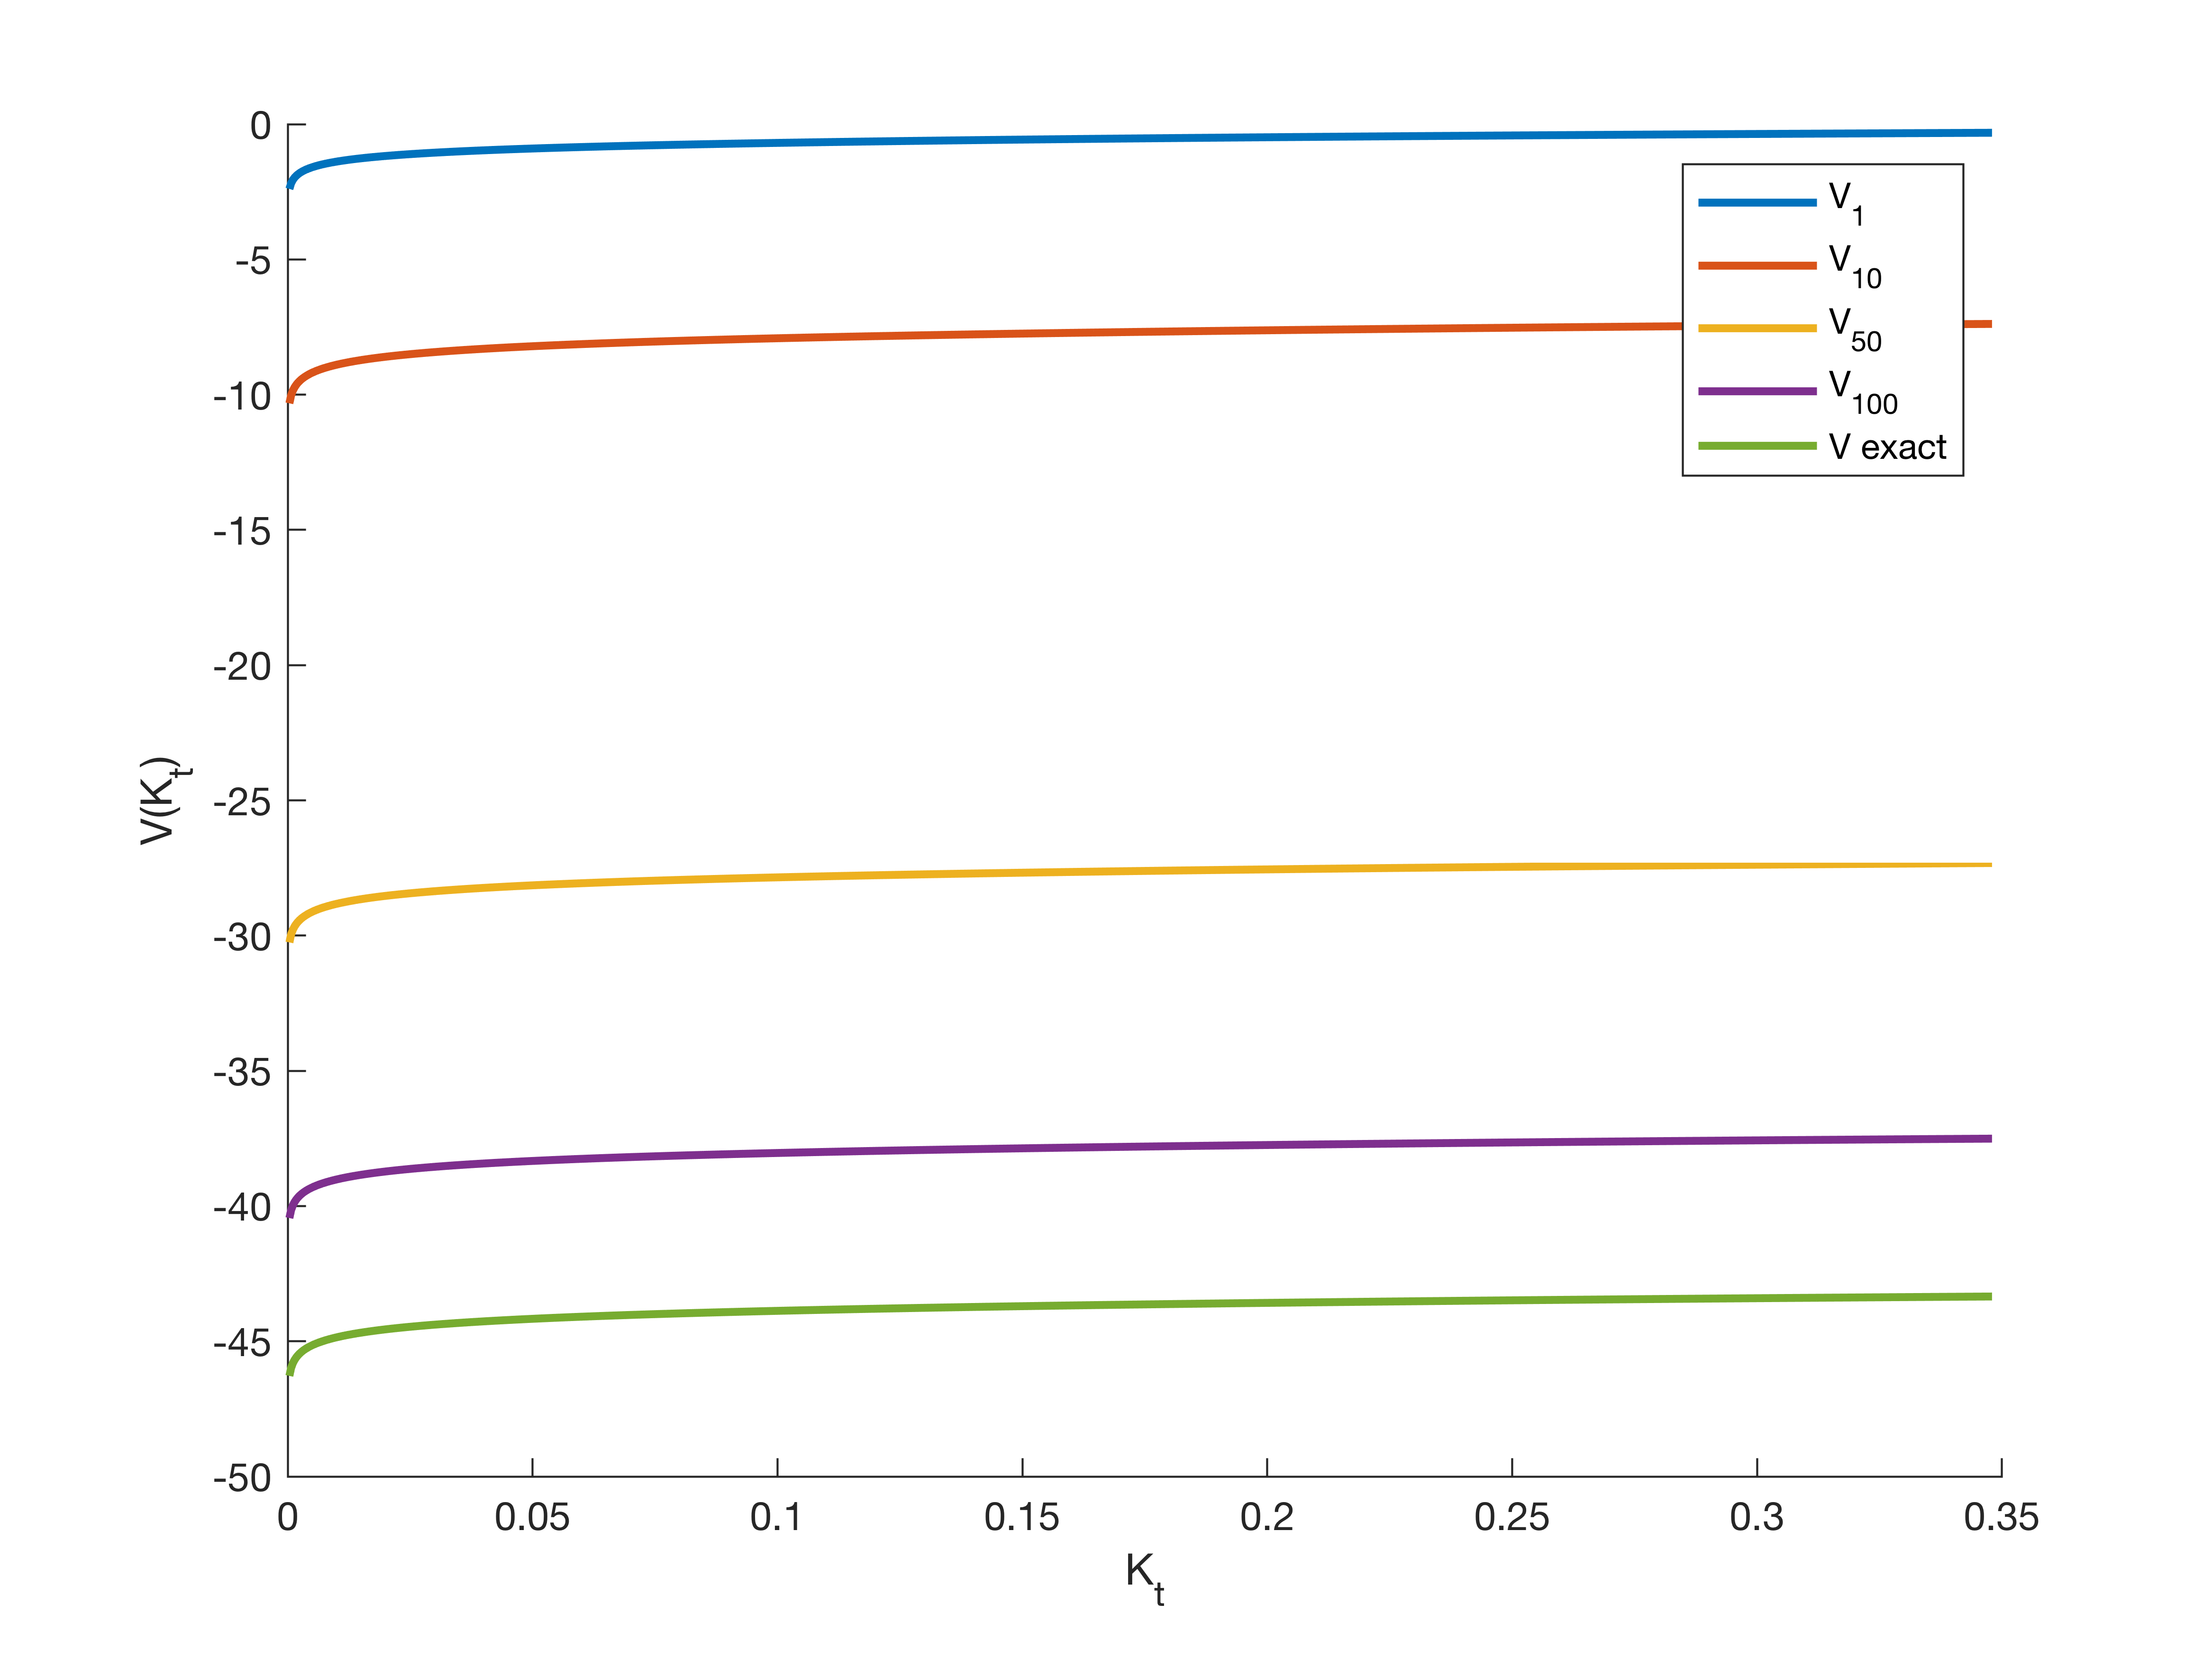
\includegraphics[width=.8\textwidth]{figure/vfi.png}
    %\includegraphics[width=2in]{XeTeX-2.jpg} 
    \caption{An Numerical Example with $\alpha = 0.3, \beta = 0.98$}
\end{figure}

Start with inital guess $V_0(K_{T+1}) = 0$
\begin{equation}
    V_1(K_T) = \begin{cases}
        \max\limits_{\{C_T, K_{T+1}\}} [u(C_T)+ \beta V_0(K_{T+1})]\\
        \quad s.t. \quad C_T + K_{T+1} = K_T^\alpha
    \end{cases}
\end{equation}
\begin{equation}
    \Longrightarrow \begin{cases}
        K_{T+1} = 0\\
        C_T =  K_T^\alpha
    \end{cases}, 
\end{equation}
Hence, $V_1(K_T) = \ln (K_T^\alpha)$. Let's continue:
\begin{equation}
    V_2(K_{T-1}) = \begin{cases}
        \max\limits_{\{C_{T-1}, K_{T}\}} [u(C_{T-1})+ \beta V_1(K_{T})]\\
        \quad s.t. \quad C_{T-1} + K_{T} = K_{T-1}^\alpha
    \end{cases}
\end{equation}
\begin{equation}
    \iff V_2(K_{T-1}) = \begin{cases}
        \max\limits_{\{C_{T-1}, K_{T}\}} u(C_{T-1})+ \beta \ln (K_T^\alpha)\\
        \quad s.t. \quad C_{T-1} + K_{T} = K_{T-1}^\alpha
    \end{cases}
\end{equation}


%===========================================================================
%===========================================================================
%===========================================================================
%===========================================================================
%===========================================================================
%===========================================================================
%===========================================================================
%===========================================================================
%===========================================================================
%===========================================================================
%===========================================================================


\section{Value function iteration}
\underline{Inital guess}: $V_0(K_{T+1}) = 0$
\begin{equation}
\Longrightarrow
    V_1(K_T) = \begin{cases}
        \max\limits_{\{C_T, K_{T+1}\}} [u(C_T)+ \beta V_0(K_{T+1})]\\
        \quad s.t. \quad C_T + K_{T+1} = K_T^\alpha
    \end{cases}
\end{equation}
Recall that $K_{T+1} = 0$ because it is the last period.
\begin{equation}
    \Longrightarrow \begin{cases}
        K_{T+1} = 0\\
        C_T =  K_T^\alpha
    \end{cases}
\end{equation}
Plugging (3.2) into (3.1),  we get
\begin{equation}
    V_1(K_T) = \ln (K_T^\alpha).
\end{equation}
Let's continue:
\begin{eqnarray}
    V_2(K_{T-1}) &=& \begin{cases}
        \max\limits_{\{C_{T-1}, K_{T}\}} [u(C_{T-1})+ \beta V_1(K_{T})]\\
        \quad s.t. \quad C_{T-1} + K_{T} = K_{T-1}^\alpha
    \end{cases}
    \\
    \Longrightarrow
    V_2(K_{T-1}) &=& \begin{cases}
        \max\limits_{\{C_{T-1}, K_{T}\}} u(C_{T-1})+ \beta \ln (K_T^\alpha)\\
        \quad s.t. \quad C_{T-1} + K_{T} = K_{T-1}^\alpha
    \end{cases}
\end{eqnarray}
\begin{equation}
    \mathcal{L} = \ln C_{T-1} + \beta \ln (K_T^\alpha) + \lambda [K_{T-1}^\alpha - C_{T-1} - K_{T}]
\end{equation}
\underline{FONC}
\begin{eqnarray}
    \frac{1}{C_{T-1}} - \lambda = 0\\
    \beta (\frac{1}{K_t^\alpha})(\alpha K_T^{\alpha-1}) - \lambda = 0   
\end{eqnarray}
\begin{eqnarray}
    \Longrightarrow
    \lambda &=& \frac{\alpha \beta}{K_T}\\
    \lambda &=& \frac{1}{C_{T-1}}\\
    \frac{\alpha \beta}{K_T} &=& \frac{1}{C_{T-1}} \quad \text{or} \quad C_{T-1} = \frac{K_T}{\alpha \beta}
\end{eqnarray}
\underline{Plug it into the constraint}
\begin{eqnarray}
    \frac{K_T}{\alpha \beta} + K_T = K_{T-1}^\alpha \\
    \Longrightarrow K_T = \frac{\alpha \beta}{1+\alpha \beta} K_{T-1}^\alpha 
\end{eqnarray}
\begin{equation}
    C_{T-1} = \frac{K_T}{\alpha \beta} = \frac{1}{\cancel{\alpha \beta}} \frac{\cancel{\alpha \beta}}{1+\alpha \beta} K_{T-1}^\alpha = \frac{1}{1+\alpha \beta} K_{T-1}^\alpha 
\end{equation}
Plug (3.12) and (3.14) into (3.5)
\begin{eqnarray}
    V_2(K_{T-1}) 
    &=& \max\limits_{\{C_{T-1}, K_{T}\}} u(C_{T-1})+ \beta \ln (K_T^\alpha) \quad \text{s.t.}~...\\
    &=& \ln( \frac{1}{1+\alpha \beta} K_{T-1}^\alpha ) + \beta \ln[\frac{\alpha \beta}{1+\alpha \beta} K_{T-1}^\alpha ]^\alpha\\
    &=& \alpha \beta \ln \alpha \beta - (1+ \alpha \beta) \ln (1+ \alpha \beta) + (1+ \alpha \beta) \ln K_{T-1}^\alpha
\end{eqnarray}
\begin{eqnarray}
    V_3(K_{T-2}) &=& \begin{cases}
        \max\limits_{\{C_{T-2}, K_{T-1}\}} [u(C_{T-2})+ \beta V_2(K_{T-1})]\\
        \quad s.t. \quad C_{T-2} + K_{T-1} = K_{T-2}^\alpha
    \end{cases}\\
    &\vdots&
\end{eqnarray}
It turns out that this sequence of value functions converges to:
\begin{equation}
    V(K_t) = \frac{\beta}{1- \beta}[\ln (1-\alpha \beta) + \frac{\alpha \beta}{1- \alpha \beta}\ln \alpha \beta] + \frac{\alpha}{1- \alpha \beta} \ln K_t
\end{equation}
To check if this limit function is indeed a solution, we plug it into the the Bellman equation (of the infinite horizon model):
\begin{equation}
    V(K_t) = \max \bigg \{ \ln C_t + \frac{\beta}{1- \beta}[\ln (1-\alpha \beta) + \frac{\alpha \beta}{1- \alpha \beta}\ln \alpha \beta] + \frac{\alpha \beta}{1- \alpha \beta} \ln K_{t+1} \bigg \} \quad s.t. \quad C_{t} + K_{t+1} = K_{t}^\alpha
\end{equation}
Recall
\begin{equation}
    \frac{1}{C_t} = \beta V'(K_{t+1}) \Longrightarrow \frac{1}{ \beta C_t } = V'(K_{t+1}) =  \frac{\alpha}{1- \alpha \beta} \frac{1}{K_{t+1}}~~\text{(by taking the derivative of (3.20))}
\end{equation}
Hence
\begin{equation}
    \frac{C_t}{K_{t+1}} = \frac{1- \alpha \beta}{\alpha \beta}
\end{equation}
Using the constaint $C_t + K_{t+1} = K_t^\alpha$,
we can get
\begin{equation}
    \frac{K_t^\alpha - K_{t+1}}{K_{t+1}} = \frac{1- \alpha \beta}{\alpha \beta} 
\end{equation}
\begin{equation}
    \Longrightarrow \text{saving rate} = \frac{K_{t+1}}{K_t^\alpha} = \alpha \beta
\end{equation}
same as old.








